\begin{frame}
\frametitle{O que é \LaTeX{}?}
\framesubtitle{}
\begin{itemize}
  \item \LaTeX{} é uma linguagem de marcação e um sistema de preparação de documentos utilizando a formatação de texto do programa \TeX{} (para se escrever com \LaTeX{} adota-se uma abordagem diferente dos processadores de texto WYSIWYG).
  \item \TeX{} é um sistema de formatação de textos projetado com dois objetivos principais:
  \begin{enumerate}
      \item permitir que qualquer um possa produzir textos de \textbf{alta qualidade} com um esforço aceitável;
      \item fornecer um sistema que gere \textbf{exatamente o mesmo resultado} em todos os computadores, agora e no futuro.
  \end{enumerate}
\end{itemize}
\end{frame}


\begin{frame}
\frametitle{\TeX{}}
\framesubtitle{}
\begin{itemize}
  \item \TeX{} é um sistema de tipografia criado no final da década de 70 por Donald Knuth (Stanford University) para a formatação da segunda edição do segundo volume de \textit{The Art of Computer Programming}.
\end{itemize}
\end{frame}
\note{
a partir da versão 3 o projeto foi congelado e só são lançadas correções de bugs. Os números das versões subsequentes aproximam assintóticamente $\pi$ (a versão atual, Março de 2008, é de número 3.1415926)

Knuth oferece um prêmio para quem encontrar Bug em seu código (valor inicial U\$2.56, dobrando a cada ano até atingir o valor atual U\$327.68)
}
\note{
When the first volume of Knuth's The Art of Computer Programming was published in 1969, it was typeset using hot metal type set by a Monotype Corporation typecaster with a hot metal typesetting machine from the 19th century which produced a "good classic style" appreciated by Knuth. When the second edition of the second volume was published, in 1976, the whole book had to be typeset again because the Monotype technology had been largely replaced by photographic techniques, and the original fonts were no longer available. However, when Knuth received the galley proofs of the new book on 30 March 1977, he found them awful. Around that time, Knuth saw for the first time the output of a high-quality digital typesetting system, and became interested in digital typography. The disappointing galley proofs gave him the final motivation to solve the problem at hand once and for all by designing his own typesetting system. On May 13, 1977, he wrote a memo to himself describing the basic features of TeX.
}
\note{
Even though Donald Knuth himself has suggested a few areas in which TeX could have been improved, he indicated that he firmly believes that having an unchanged system that will produce the same output now and in the future is more important than introducing new features. For this reason, he has stated that the "absolutely final change (to be made after my death)" will be to change the version number to π, at which point all remaining bugs will become features.
}


\begin{frame}
\frametitle{\LaTeX{}}
\framesubtitle{}
\begin{itemize}
  \item \LaTeX{} é um conjunto de macros para o \TeX{} desenvolvido na década de 80 por Leslie Lamport.
  \item Amplamente utilizado no meio acadêmico, principalmente nas seguintes áreas: matemática, ciência da computação, engenharia, física, estatística e psicologia quantitativa.
\end{itemize}
\end{frame}



\begin{frame}
\frametitle{Licença}
\framesubtitle{}
\begin{itemize}
  \item \TeX{} possui licença de software permissiva (BSD-like).
  \item \LaTeX{} poussi licença própria: \LaTeX{} Project Public License (LPPL).
\end{itemize}
\end{frame}


\begin{frame}
\frametitle{Por que utilizar \LaTeX{}?}
\framesubtitle{}
\begin{itemize}
  \item portabilidade - Linux, Mac OS, Windows, BSDs, Solaris, etc.
  \item compatibilidade - padrão imutável
  \item flexibilidade
  \item controle
  \item apresentação, elegância
  \item fórmulas, tabelas, figuras
  \item disseminado (principalmente no meio academico)
  \item estabilidade
  \item livre
\end{itemize}
\end{frame}

\begin{frame}
\frametitle{\LaTeX{} vs Word}
\framesubtitle{Devo utilizar \LaTeX{} ao invés do Word ou LibreOffice?}
  \begin{figure}[h!]
  \centering
  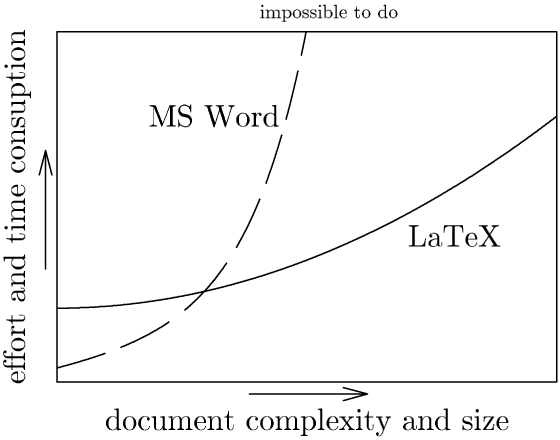
\includegraphics[width=0.7\textwidth]{figures/word_vs_latex.png}
  \caption{\LaTeX{} vs Word.}
  \label{fig:word_vs_latex}
  \end{figure}
\end{frame}

\begin{frame}
\frametitle{Onde aprender \LaTeX{}?}
\framesubtitle{Hoje é muito mais fácil utilizar e aprender qualquer coisa.}
\begin{itemize}
  \item \hrefcolor{http://www.ctan.org/tex-archive/info/lshort/english/lshort.pdf}{The Not So Short Introduction to LaTeX2e}
  \item \hrefcolor{http://www.sbm.org.br/periodicos/latexemportugues.pdf}{Breve Introdução ao LATEX2e}
  \item Google Groups: \hrefcolor{https://groups.google.com/forum/\#!forum/comp.text.tex}{comp.text.tex}
  \item a
\end{itemize}
\end{frame}

\begin{frame}
\frametitle{\LaTeX{}}
\framesubtitle{}
\begin{itemize}
  \item
\end{itemize}
\end{frame}